% Chapter 2

\chapter{Methods and Models} % Main chapter title

\label{Chapter2} % For referencing the chapter elsewhere, use \ref{Chapter1} 

\lhead{Chapter 2. \emph{Methods and Models}} % This is for the header on each page - perhaps a shortened title

%----------------------------------------------------------------------------------------

In this section, the construction of brain graphs based on empirical functional connectivity matrix (FCM) and anatomical connectivity matrix (ACM) will be first introduced. Then, the topological characteristics of all graphs will be statistically measured and those topological measures will be interpreted neuro-biologically. In particular, it is aimed to explore under which conditions that brain network topologies distinguish from random networks. For this purpose, tools and concepts from graph theory / network science will be used. This approach is expected to provide a deeper insight into the underlying process involved in the observed functional and structural brain connectivity. 


\textit{Graph theory} is a mathematical field applicable to a large diversity of complex systems such as markets, ecosystems, computer circuits, and gene-gene interactions \citep{XYZ09}. A graph is defined as an ensemble of vertices (nodes) that are connected by edges (links). If the edges connect the nodes in a specified direction, the graph is referred to as \textit{directed}, otherwise \textit{undirected}. Moreover, the edges can be assigned a weight yielding a \textit{weighted} graph. A graph with edges of uniform weight is called an \textit{unweighted} graph.

\textit{Network science} incorporates graph theory applied on a   
distinct complex domain. Unlike classical graph theory, network science primarily deals with real-life networks that are large and complex - neither uniformly random nor ordered \citep{RUB10}. The neuro-anatomical and neuro-physiological data sets derived from  DW-MRI and fMRI-BOLD techniques can be considered as such large-scale complex brain graphs, that can be modeled as \textit{undirected} and \textit{unweighted} networks for simplicity. Nodes in large-scale brain networks usually represent brain regions, while edges represent anatomical, functional or effective connections \citep{XYZ94}. 


A brain network can be statistically described in terms of its topology, i.e. solely in terms of its connectivity and independently of spatial positions of nodes and edges. Topological measures described in previous studies capture local and global properties of a network, e.g. local and global efficiency, clustering coefficient, transitivity and small-worldness \citep{LAT01, WAT98, NEW03, HUM08}.


Methods of graph theory applied to structural and functional systems have shown that both share typical features of many complex networks \citep{BUL09, RUB09, HEU11, VUK14}. However, the essential features of brain's connectivity still remain ambiguous both for functional and structural maps. This project aims to investigate whether or not the brain behaves as a completely random circuitry. This idea will be tested by comparing brain graphs to the randomized networks as it was previously noticed by Bullmore and Bassett \citep{BUL11a}. The majority of random graphs here are inspired by  Erd\H{o}s-R\'{e}nyi-type random networks and the configuration model. 
 

The following subsections will introduce building real-networks given empirical brain connectivity maps, generating random networks by manipulating the brain graphs with randomization procedures and quantifying the spatial characteristics of all graphs constructed. Once the graph theory related methods are covered, the temporal dynamics for the neuronal activity and BOLD fluctuations will be explained in further subsections of Chapter 2. 



\section{Empirical Brain Connectivity Maps}

The functional-magnetic-resonance-imaging (fMRI) is a widely used method to detect the blood oxygen level dependent (BOLD) contrast in the brain. The fMRI-BOLD contrast is used to interpret the neuronal activity in the respective voxel, which can be considered as a rectangular volume in brain defined for the imaging studies. The ongoing firing activity of neurons requires energy and it is supplied by neighboring blood cells via oxygen and glucose release into the nerve cells. The deviations in deoxygenation level, cerebral flow and volume in blood vessels due to neuronal activity, known as \textit{hemodynamic process}, cause a change in the detected fMRI-BOLD signal strength. The functional connectivity matrix (FCM) represents correlation coefficients of these fMRI-BOLD signals detected from the pre-defined brain regions with voxels. 

The resting state empirical FCM used in this project is obtained from the \textit{1000 Functional Connectome Project} website \url{http://www.nitric.org/}). The human brain is segmented into $N=90$ cortical and sub-cortical regions according to the Tzourio-Mazoyer brain atlas with the automated anatomical labeling (AAL) template  \citep{TZO02}, such that regions with index $n=\{1,2,...,45\}$ lie on the right hemisphere, whereas $n=\{46,47,...,90\}$ are on the left (Appendix A). The fMRI-BOLD activity is measured from all voxels in an AAL region for 7.5 min of acquisition time. Once the fMRI-BOLD mean time-series are obtained for all AAL regions, the FCM is obtained by calculating the Pearson correlation coefficients of time-series between all pairs of the 90 AAL regions. Therefore the size of FCM is $N\times N = 90 \times 90$.  To be more precise, BOLD-fMRI signal is averaged for the same subject over voxels in an AAL region, and FCM is averaged over all subjects at the end. 

The diffusion weighted magnetic resonance imaging (DW-MRI) technique estimates the anatomical connection probabilities among brain regions by investigating the diffusion direction of water molecules within a voxel. The direction of the fiber tracks in white matter depends on the diffusion pattern of water molecules. A DW-MRI experiment approximates the existence of a fiber track between regions of interest. The anatomical connectivity matrix (ACM) used in this project is obtained from the study of Iturria-Medina et al. \citep{ITU08} and it is based on the same $N=90$ AAL regions as in the FCM described above. The size of ACM is also $N\times N = 90\times 90$, and each value reveals the probability of 2 AAL regions being connected via axonal fibers. 
  
\begin{figure}[htbp]
 
  \centering
	 \includegraphics[width=0.49\textwidth]{Figures/cor_FCM_exp.eps} 
	 \includegraphics[width=0.49\textwidth]{Figures/cor_ACM_exp.eps} 
	
    \rule{35em}{0.5pt}
  \caption[Empirical FCM and ACM]{Empirical functional and anatomical connectivity maps of human cortex, FCM obtained from fMRI-BOLD technique (on the left) and ACM obtained from DW-MRI (on the right). The colorbars exhibit correlation coefficients and probability values in FCM and ACM, respectively. }
  \label{fig:Empirical FCM and ACM}
 	
\end{figure}  

 
\begin{figure}[htbp]
 
  \centering
	 \includegraphics[width=0.49\textwidth]{Figures/FCM_brain.eps} 
	 \includegraphics[width=0.49\textwidth]{Figures/ACM_brain.eps} 
    \rule{35em}{0.5pt}
  \caption[Empirical FCM and ACM in Cortex]{3D sagittal visualization of empirical FCM (on the left) and ACM (on the right) on the human cortex with the \textsc{BrainNet Viewer}. The colorbars are the same as explained in Figure 2.1. \citep{XYZ13}. } 
  \label{fig:Empirical FCM and ACM in Cortex}
 	
\end{figure} 

Figure 2.1 represents empirically captured FCM and ACM. All correlation coefficients in FCM appear in the range [0,1] as well as all probability values in ACM. Both matrices are symmetric. A correlation value close to 1 in FCM indicates that the quantified functional activities of corresponding nodes in the right and left hemisphere highly resemble each other (see sub-diagonals in Figure 2.1, left). A probability value close to 1 in ACM demonstrates that corresponding nodes are most likely connected by fiber tracks in white matter. Although some node pairs are not anatomically coupled at all in ACM (cold colors), they could be functionally coupled in FCM (hot colors). This is especially true for the corresponding regions in the different hemispheres.    

FCM and ACM are embedded in human cortex in Figure 2.2 \citep{XYZ13}. All nodes are presented with equal size and black color independent of their topological properties. However, edges have different thickness and color distribution according to correlation coefficients and probability values with respect to FCM and ACM. 
 
   
\section{The Brain Graph}

The brain graphs considered here are derived from two sets of empirical brain connectivity maps: FCM and ACM obtained from fMRI-BOLD and DW-MRI techniques, respectively. Those data sets represent measurements from $N=90$ cortical and sub-cortical regions labeled with AAL, represented by nodes in the graph. The nodes can be connected to each other by means of \textit{edges}. If the graph is constructed on the FCM, edges are interpreted as correlation strengths between the functional BOLD activity of two nodes. If the graph is built on the ACM, an existing edge is considered as the probability of two nodes to be structurally connected by fiber tracks in white matter.

The brain graphs in this project are generated through binarizing the functional connectivity matrix (FCM) and anatomical connectivity matrix (ACM). Binarization here means converting all the values in a given matrix into 1's and 0's via thresholding. Because of the nature of their definition, both empirical data sets have values between 0 and 1, reflecting a correlation strength in case of FCM or a probability value in case of ACM. We arbitrarily define a threshold value $r$ for the strength of correlations in FCM. Then, the values greater and equal to $r$ are assigned the value 1, while others are set to 0. This thresholding is applied by means of the strength of probability value, $p$, for the ACM. The binarized matrix is the basis of brain graph construction, and it is commonly known as \textit{adjacency matrix}. The \textsc{NetworkX} software package in \textsc{PYTHON} is used to built graphs given adjacency matrices \citep{XYZNETW}. Neither the direction of functional or anatomical connectivity between nodes, nor any other values apart from 0 and 1  are encoded in the adjacency matrices  so that the resulting graphs are considered as \textit{undirected} and \textit{unweighted}. In other words, all existing edges are thought to be of uniform weight and nodes interact both ways along an edge connecting them. 

\begin{figure}[htbp]
 %\begin{tabular}{cc}
  \centering
	 \includegraphics[width=0.45\textwidth]{Figures/cor_FCM_exp.eps} 
	 \includegraphics[width=0.45\textwidth]{Figures/Sample_Adj.eps} 
	\includegraphics[width=0.45\textwidth]{Figures/Sample_Adj_brain.eps}  
   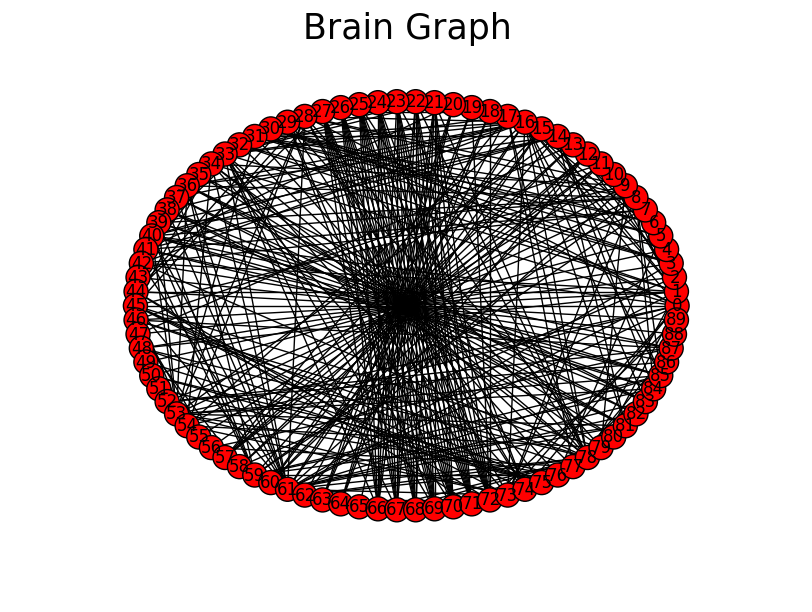
\includegraphics[width=0.45\textwidth]{Figures/brain_graph.png}      

    \rule{35em}{0.5pt}
  \caption[Binarizing via thresholding]{How to build a brain graph: The empirical data matrix derived from fMRI-BOLD technique (upper left) is binarized via a threshold value $r=0.55$ and its corresponding adjacency matrix (upper right). The black spots represent 1's indicating edges between nodes, whereas the white squares represent 0's implying no edge. The adjacency matrix is embedded on human cortex axially (lower left) with \textsc{BrainNet Viewer} \citep{XYZ13} and the brain graph derived from the adjacency matrix with \textsc{NetworkX} \citep{XYZNETW}(lower right).}
  \label{fig:Binarizing via thresholding}
 %\end{tabular}	
\end{figure}

Figure 2.3 illustrates the exemplary construction of a brain graph from the FCM. All correlation values among the cortical and sub-cortical regions in the empirical fMRI-BOLD data lie between 0 and 1. The 3D axial cortex visualization represents only the existing edges with black edges among the nodes. The adjacency matrix (AM) is filled out only with 1's and 0's indicating functionally connected and unconnected nodes, whose correlated BOLD activity is equal to or greater than $r=0.55$. The algorithm \textsc{Networkx} builds the corresponding brain graph of an adjacency matrix \citep{XYZNETW}. The AM obtained from an ACM would look similar, but would represent the probability of two nodes to be anatomically connected above a predefined threshold $p$. 

The following sections will cover randomization methods reshuffling the brain graphs and introduce some of the topological concepts characterizing brain graphs as well as random networks.



\section{Randomization Methods}





\subsection{Erd\H{o}s-R\'{e}nyi-Type Randomization}

Given a total number of nodes $N$, Paul Erd\H{o}s and Alfr\'{e}d R\'{e}nyi produced an undirected graph $G(N,P)$, in which the presence of any edge between two nodes is assigned a probability $P$. 
The average total number of edges $L$ in an  Erd\H{o}s-R\'{e}nyi-type random graph is $\binom {N} {2}P$, with a binomial distribution for the number of edges per node, known as the \textit{degree} of a node \citep{XYZERD}. 

New randomization techniques arise through modifying the Erd\H{o}s-R\'{e}nyi method, e.g. given $N$ and $L$, a graph $G(N,L)$ can be picked uniformly random out of the set of all potential graphs having $N$ nodes and $L$ edges, which means the same network \textit{density}. The probability for a graph to be picked among all the others is $\frac{L}{\binom {N}{2}}  $. One can study the various aspects of $G(N,P)$ and $G(N,L)$ even more detailed, but for the sake of simplicity, Erd\H{o}s-R\'{e}nyi model will not be discussed further here \citep{XYZERD, NEW10}.

\begin{figure}[htbp]
 %\begin{tabular}{cc}
  \centering
	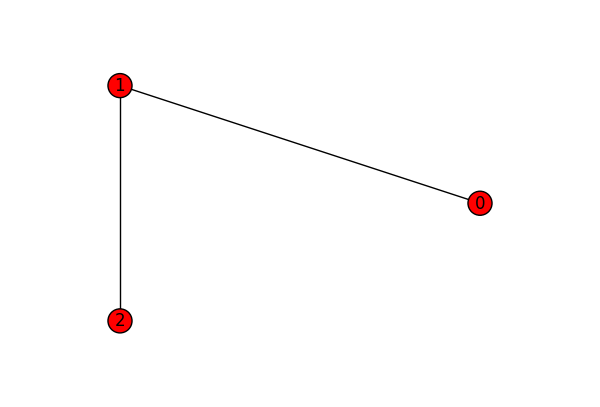
\includegraphics[width=0.30\textwidth, height=40mm]{Figures/f1.png}  
	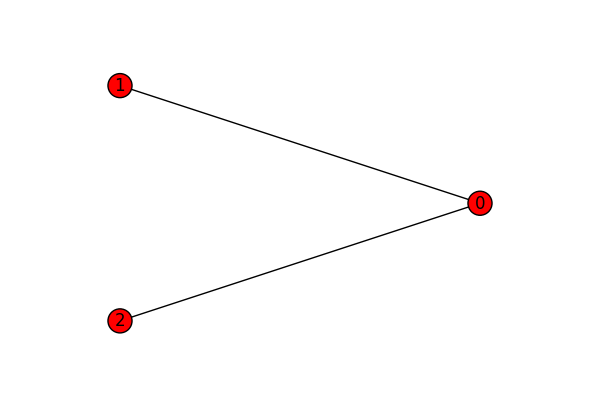
\includegraphics[width=0.30\textwidth, height=40mm]{Figures/f2.png} 
    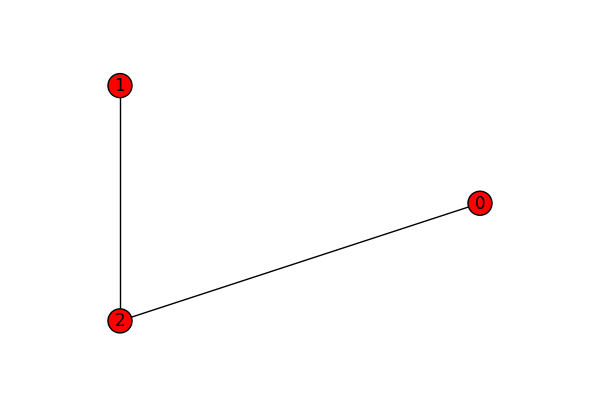
\includegraphics[width=0.30\textwidth, height=40mm]{Figures/f3.png}

    \rule{35em}{0.5pt}
  \caption[Erdos-Renyi Example]{An illustration of the set of all $G(N,L)$ type random graphs with $N=3$ and $L=2$.}
  \label{fig:Erdos-Renyi Example}
 %\end{tabular}	
\end{figure}

Figure 2.4 illustrates all possible graphs having 3 nodes and 2 edges. One of those 3 simple graph is chosen uniformly random for the $G(N,L)$ randomization type, so that each graph is chosen with probability $P=\dfrac{1}{3}$.  

The $G(N,L)$ type randomization is the first method used to derive random graphs from the adjacency matrices of FCM and ACM in this project. Both matrices have $N=90$ nodes. However $L$ changes for each brain graph according to the applied threshold level and therefore is always recalculated. 

\subsection{Double-Edge-Swap Type Randomization}

The \textit{degree} $k_i$ of a node $i$ is defined as the number of edges connected to that node. The double-edge-swap method manipulates a given graph by swapping two existing edges among four nodes, while keeping the node degrees fixed. 


\begin{figure}[htbp]
 %\begin{tabular}{cc}
  \centering
	\includegraphics[width=0.32\textwidth, height=50mm]{Figures/G1_swap.eps}  
    \includegraphics[width=0.32\textwidth, height=50mm]{Figures/G2_swap.eps}  
	\includegraphics[width=0.32\textwidth, height=50mm]{Figures/G3_swap.eps} 
    \rule{35em}{0.5pt}
  \caption[Double-Edge-Swap Example]{Swapping edges between 2 paired nodes.}
  \label{fig:Double-Edge-Swap Example}
 %\end{tabular}	
\end{figure}

Figure 2.5 illustrates randomly chosen double edges in a sample graph to be swapped. After the existing edges are removed, the new pair of nodes are rewired. The degree of each node is the same before and after swapping; degrees of nodes $k_1 = 1$, $k_2=1$, $k_3=1$, $k_4=1$ are all fixed in each graph. Although the randomly constructed graphs with the double-edge-swap method are expected to have same degrees, the latter is not a unique property identifying a graph.

The \textit{degree distribution} is the probability distribution of node degrees over the whole graph. Conservation of each $k_i$ preserves the degree distribution, however, preserving degree distribution does not guarantee to fix $k_i$ values. We will discover in the next section how to preserve degree distribution by altering node degrees.

\subsection{Preserved-Degree-Distribution Type Randomization}

The preserved-degree-distribution method randomizes a given network by rewiring its edges while recovering its degree distribution $p(k)$. The sum of degree distributions and cumulative distribution $P(k')$  can be stated algebraically with the following equation,

\begin{equation}
1= \sum{p(k)}, \,\,\,\,\,\,\,\,\,\,\,   P(k') = \sum_{k \geq k'} p(k),
\end{equation}

where $p(k)$ is the probability of a node to have degree number $k$ \citep{BAR99a}.


\begin{figure}[htbp]
 %\begin{tabular}{cc}
  \centering
	\includegraphics[width=\textwidth, height=60mm]{Figures/G_degree_dist_1.eps}  
	%\includegraphics[width=0.45\textwidth, height=60mm]{Figures/G_degree_dist_2.eps}    
    \rule{35em}{0.5pt}
  \caption[Degree Distribution 2D Example]{A sample graph (left) and its randomized version (right) with preserved-degree-distribution method. $p(k=1)=\frac{1}{5}$, $p(k=2)=\frac{3}{5}$, and $p(k=3)=\frac{1}{5}$ in both graphs. }
  \label{fig:Degree Distribution Example}
 %\end{tabular}	
\end{figure}

The algorithm for the preserved-degree-distribution is adapted from \textit{Brain Connectivity Toolbox} (\textsc{BCT}) \citep{XYZBCT}. Figure 2.6 demonstrates a sample graph and its randomized version via preserved-degree-distribution method. Not only the $p(k)$, but also the individual node degrees $k_{i}$ do not go under any change.  The algorithm resembles highly the double-edge-swap type randomization tool implemented from \textsc{NetworkX} \citep{XYZNETW}. However, it ensures that the graph stays \textit{connected}, i.e. it is always possible to reach a node through any other node in the graph. 

\begin{figure}[htbp]
 %\begin{tabular}{cc}
  \centering
	\includegraphics[width=\textwidth]{Figures/G_degree_dist.eps}  
    \rule{35em}{0.5pt}
  \caption[Degree Distribution 3D Example]{Heat maps for degree distributions of the brain graph (obtained from functional connectivity map of brain, fMRI-BOLD data) (left), and of the randomized graph with preserved-degree-distribution tool (right). Colorbars are in logarithmic scale.}
  \label{fig:Degree Distribution 3D Example}
 %\end{tabular}	
\end{figure}

$p(k)$ is a global topological measure for a network, it can be illustrated over all nodes in the whole graph as in Figure 2.7. Node indices are labeled on $x$-axis of the heat map, threshold $r$ values for adjacency matrices are given on $y$-axis. The preserved-degree-distribution method generates successfully a random graph with the same $p(k)$ as in the brain graph. 


\subsection{Configuration Model Randomization}

The \textit{degree sequence} of a graph is either its ascending or descending sequence of node degrees. The configuration model generates a random graph with a given degree sequence. The direct implementation of this model is to assign edges to the nodes randomly until the desired degree sequence is matched. The resulting random graph is expected to be a node-index-shuffled version of the original graph. However, these algorithms are non-trivial due to the occurrence of self-loops (node is connected to itself) and parallel edges (multiple edges connecting two nodes), which are both undesirable graph properties in this project. 

\begin{figure}[htbp]
 %\begin{tabular}{cc}
  \centering
	\includegraphics[width=0.45\textwidth, height=60mm]{Figures/G_config_1.eps}  
	\includegraphics[width=0.45\textwidth, height=60mm]{Figures/G_config_2.eps} 
    \rule{35em}{0.5pt}
    \caption[Degree Sequence Definition]{The degrees of the nodes in the original graph (left): $k_0 = 2$, $k_1 =1$, $k_2=2$, $k_3=3$ and that of the randomized graph (right): $k_0 = 3$, $k_1 =2$, $k_2=1$, $k_3=2$. The degree sequence in non-increasing order in both graphs: $\{3,\,2,\,2,\,1\}$}
  \label{fig:Degree Sequence Definition}
 %\end{tabular}	
\end{figure}

Figure 2.8 points out the relevance of the degree sequence to the node degrees. Moreover, one should not confuse degree distribution and degree sequence.   

The configuration model variant used here is the expected-degree-graph method, which excludes self-loops and parallel edges. This algorithm receives the list of the expected degree sequence as an input $(k_u, k_v, k_m, k_l, ...)$, and assigns edges between nodes with a predefined probability $P_{uv}=\dfrac{k_u k_w}{\sum_{i}k_i}$. This method does not guarantee to construct graphs with exactly the same given degree sequence but with the closest possible sequence.  



 
\subsection{Partial Randomization}
 
The partial randomization method  reconstructs a graph (say A) with partial rewirings with respect to a second graph (say B) while keeping the degree distribution the same as in A. The analogy of this algorithm is to perform rewirings in the adjacency matrix of A, while avoiding any edge generation which already exist in the B. In other words, the choice of edges to be performed rewirings in A is limited with respect to the B. 

In this project, the functional connectivity (FC) adjacency matrix is partially rewired with respect to the anatomical connectivity (AC) adjacency matrix.  This means doing such rewirings among the nodes in FCM only if these nodes are not structurally connected in the brain with probability above a given value. The same procedure is done to randomize AC adjacency matrix partially with respect to FC adjacency matrix.  This time nodes in ACM can be linked only if they are not functionally correlated above a given threshold.   

\begin{figure}[htbp]
 %\begin{tabular}{cc}
  \centering
	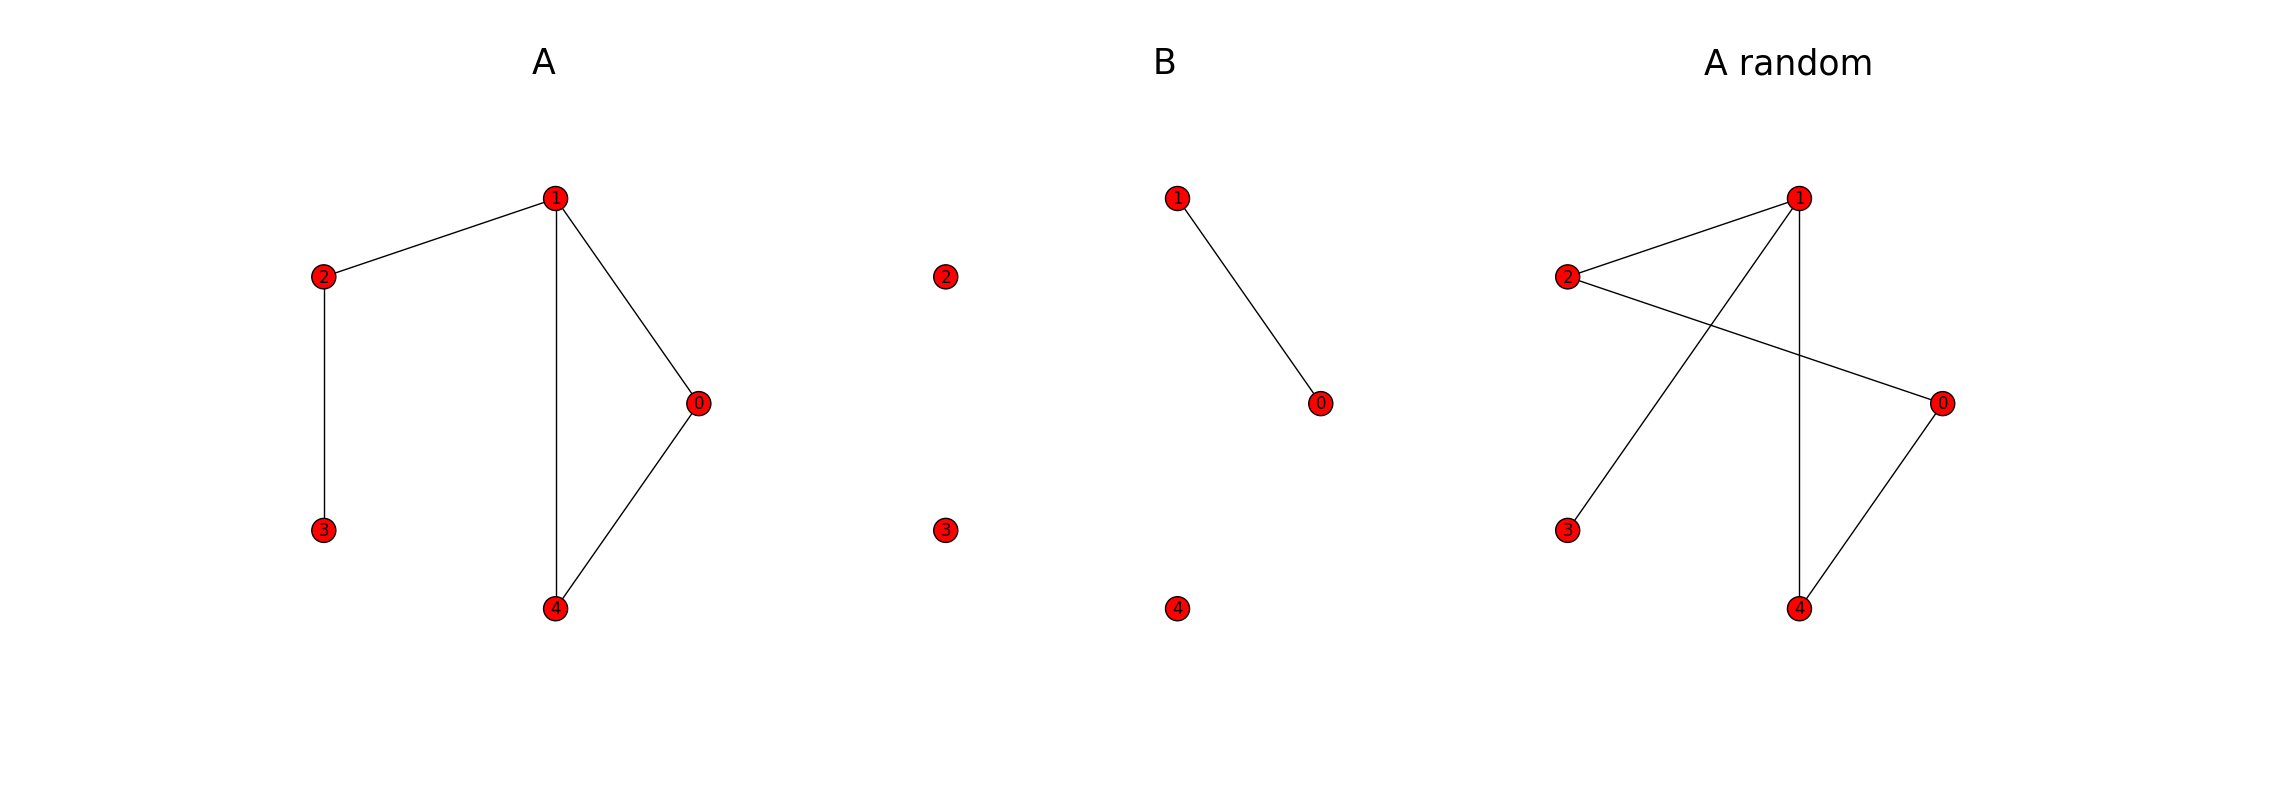
\includegraphics[width=\textwidth, height=55mm]{Figures/p1.png}  
    \rule{35em}{0.5pt}
    \caption[Partial Randomization Example]{Graph A is performed a partial randomization with respect to graph B. While the partial randomization tool rewires edges in A, it avoids creating such edges that exist in B.}
  \label{fig:Partial Randomization Example}
 %\end{tabular}	
\end{figure}

Representative graphs $A$ and $B$ in Figure 2.9 can be thought as FCM and ACM, respectively. In this case, $A \,\, random$ is the partially randomized graph of FCM with respect to ACM.


The brain graph and randomly generated graphs will be identified in terms of their topological properties in the following sections. For simplicity the abbreviations are introduced in the table below. 

\begin{table}[h]
\begin{center}
\caption[Abbreviations of Randomization Methods]{Abbreviations for the brain graph and the randomly constructed graphs. }
\begin{tabular}{ l | c | r }
  Abbreviation & Description & method \\
  \hline  \hline                     
  $R_{BG}$ & the brain graph               & \textsc{NetworkX} \citep{XYZNETW} \\ \hline
  $R_{ER}$ & Erd\H{o}s-R\'{e}nyi, G(N,L)   & \textsc{NetworkX} \citep{XYZNETW}\\ \hline
  $R_{DES}$ & double-edge-swap             & \textsc{NetworkX}\citep{XYZNETW} \\ \hline
  $R_{PDD}$ & preserved-degree-distribution& \textsc{BCT} \citep{XYZBCT}	 \\ \hline  
  $R_{CM}$ & configuration model       	   & \textsc{NetworkX} \citep{XYZNETW} \\ \hline
  $R_{PR}$ & partial randomization         & \textsc{BCT} \citep{XYZBCT}	 \\ \hline  
  \hline  
\end{tabular}
\label{table:Abbreviations of Randomization Methods}
\end{center}
\end{table}	

Section 2.1 introduced the empirical data sets used in this project; the functional connectivity (FM) map and anatomical connectivity (AM) map, which are obtained from fMRI-BOLD and DW-MRI measurements at resting state of brain. Section 2.2 brought up the construction of brain graphs based on FC and AM maps. Section 2.3 explained the randomization tools to manipulate these brain graphs topologically. The next section aims to characterize the network measures of $R_{BG}$ and all other random graphs.

\section{Network Characterizations}


A network can be statistically described in terms of its topology, i.e. solely in terms of its connectivity and independently of spatial positions of nodes and edges. Topological measures described in previous studies capture local and global properties of a network, e.g. local and global efficiency, clustering coefficient, transitivity and small-worldness \citep{LAT01, WAT98, NEW03, HUM08}. This section aims to characterize the topology of brain graphs obtained from FC and AC maps together with the topology of the random networks, which are generated by applying the randomization procedures on the brain graphs (Section 2.3).   



\subsection{Network Density}
The \textit{average degree} $\langle k \rangle$ of a network is proportional to the ratio of total number of edges $L$ to total number of nodes $N$ in a graph, 

\begin{equation}
\langle k \rangle = \frac{2L}{N}.
\end{equation}

It should be noted that in order to not count each edge twice, the total number of edges is divided by $N/2$ instead of $N$. The \textit{density} $\kappa$ of a network is a scaled version of average degree measurement. It is formulated as the ratio between $L$ and maximum number of possible edges $\binom{N}{2}$,

\begin{equation}
\kappa = \frac{2L}{N(N-1)}.
\end{equation}	

The measure of network density can be referred to as the total \textit{wiring cost} of the network \citep{RUB10}. The degree, average degree and network density are key scalar measures to characterize the topology of a network. There is, for instance, clinical evidence that reductions in nodal degree are associated with greater severity of local amyloid deposition in patients with Alzheimer's disease \citep{XYZ2009}. 

\begin{figure}[htbp]
 %\begin{tabular}{cc}
  \centering
	\includegraphics[width=0.48\textwidth, height=55mm]{Figures/Network_Density_Fnc.eps}
	\includegraphics[width=0.48\textwidth, height=55mm]{Figures/Network_Density_Stru.eps}  
    \rule{35em}{0.5pt}
    \caption[Network Density]{Network density of the brain graphs constructed on FC (left) and AM (right) maps, and their randomized networks. The abbreviations are chosen as described in Table 2.1.}
  \label{fig:Network Density}
 %\end{tabular}	
\end{figure}


The network density $\kappa$ can be considered a probability for all graphs in corresponding threshold $r$ and $p$ ranges. The random networks are built in such ways that they have the same number of nodes and almost the same $\kappa$ as in the brain graphs. However, the $\kappa$ is not a unique metric identifying a network.

Figure 2.10 shows that all networks are densely connected for low $r$ and $p$. For the functional $R_{BG}$ and its randomized graphs, $\kappa$ decreases sigmoidally with $r$. In comparison, $\kappa$ decreases very sharp at low $p$, which is followed by smooth decay at intermediate $p$ for the anatomical  $R_{BG}$ and its randomized networks. It should be noted that all graphs have almost the same $\kappa$ values. 

Functional networks are likely to be denser than anatomical networks, as they will typically contain numerous connections between anatomically unconnected regions \citep{DAM09}. 

\subsection{Average Clustering Coefficient}
    
The \textit{average clustering coefficient} $C$ of a network is calculated through individual clustering coefficients $C_i$ of single nodes,

\begin{equation}
C = \frac{1}{n} \sum\limits_{i\epsilon N}C_i = \frac{1}{n}\sum\limits_{i\epsilon N} \frac{2t_i}{k_i(k_i -1)} .
\end{equation} 

where $t_i$ is the number of triangles around node $i$ and $k_i$ is the degree of node $i$ \citep{WAT98}. The clustering coefficient is a measure of segregation, that is, the ability for specialized processing to occur within densely interconnected groups of brain regions \citep{RUB10}. It reveals how the individual nodes in a graph cluster together; how many neighbors of a node are neighbors of each other. 

\begin{figure}[htbp]
 %\begin{tabular}{cc}
  \centering
	\includegraphics[width=0.48\textwidth, height=55mm]{Figures/Clustering_Coefficient_Fnc.eps}
	\includegraphics[width=0.48\textwidth, height=55mm]{Figures/Clustering_Coefficient_Stru.eps} 
    \rule{35em}{0.5pt}
    \caption[Clustering Coefficient]{Average clustering coefficient of the functional (left) and anatomical (right) brain graphs and their randomized networks. }
  \label{fig:Clustering Coefficient}
 %\end{tabular}	
\end{figure}

The clustering coefficient $C_i$ of a node $i$ is a measure of local connectivity and is highly correlated with the local efficiency of the information transfer \citep{LAT01}. The $C_i$ is formulated as the ratio of $t_i$ over all possible edges of the node $i$; $\binom{k_i}{2} $. The average clustering coefficient $C$ is a normalized version of $C_i$ for the whole network, yielding now a global property. All $C$ values are between 0 and 1. Figure 2.11 shows that at lower binarization thresholds, nodes tend to cluster more due to a higher number of existing edges. The empirically obtained brain networks of FC and AC maps have the highest $C$ compared to random graphs. The local information transfer seems to be more efficient in the brain graphs.  The randomized graphs $R_{ER}$, $R_{DES}$, $R_{CM}$, $R_{PDD}$ and $R_{PR}$ (Figure 2.11, right) share more nodes with lower degrees compared to the anatomical $R_{BG}$.

\subsection{Transitivity}

Transitivity is a similar measure to the clustering coefficient, and also quantifies segregation in the network. It is defined as \citep{NEW03}
	
\begin{equation}
 T = \frac{2\sum\limits_{i \epsilon N}  t_i}{\sum\limits_{i \epsilon N}k_i (k_i - 1)} .
\end{equation}	

If a node has links to two other nodes, transitivity inquires whether those two other nodes are also connected to each other. It asks, what percentage of triangles in the network is closed. Transitivity resembles clustering coefficient, however, it is defined only for the whole network rather than single nodes. 

\begin{figure}[htbp]
 %\begin{tabular}{cc}
  \centering
	\includegraphics[width=0.48\textwidth, height=55mm]{Figures/Transitivity_Fnc.eps}
	\includegraphics[width=0.48\textwidth, height=55mm]{Figures/Transitivity_Stru.eps} 
    \rule{35em}{0.5pt}
    \caption[Transitivity]{Transitivity of the brain graphs and random graphs of FCM (on the left) and ACM (on the left). }
  \label{fig:Transitivity}
 %\end{tabular}	
\end{figure}


The degree of transitivity is one of the fundamental differences between real world networks and random networks \citep{NEW10}. This difference is more pronounced than the clustering difference between brain graphs and random graphs, especially for the FC map related graphs when Figures 2.11 and 2.12 are compared. $T$ is more effected by the degree distribution $p(k)$ of a network, the more nodes with lower degrees, the higher the value of $T$ is. AC related graphs tend to have lower $p(k)$ values distributed among many nodes, whereas FC related graphs have higher $p(k)$ values distributed among less nodes. This holds even for $R_{BG}$ and $R_{PDD}$ graphs of FCM in Figure 2.12, and their $p(k)$ is reflected in higher $T$ (Appendix B).

Section 2.4 demonstrated exemplary statistical measures used to identify networks. Other topology measures, i.e. $p(k)$ of networks, assortativity, small-worldness, local and global efficiency, are illustrated in Appendix B. The next section will introduce the modeling approach for the neuronal activity in each brain node.   



\section{FitzHugh-Nagumo Model for Neuronal Activity Simulation}

An fMRI-BOLD experiment reveals the correlation coefficients between timeseries of BOLD activity among pre-defined brain regions. The empirical functional connectivity matrix (FCM) derived from fMRI-BOLD technique in this project reflects those coefficients among $N=90$ AAL regions at the resting state of the human brain, i.e. no stimulus is introduced to the subject. Despite the lack of any stimulus, the observed fMRI-BOLD signal in the mammalian brain is highly structural and robust at low frequency fluctuations ($<$0.1 Hz) \citep{BIS95, DAM06, VIN07a}. However, the underlying reason of these well organized spatio-temporal dynamics has not yet been completely resolved. The existing models of resting-brain dynamics hypothesize that functional interactions result from a complex interplay between intrinsic brain dynamics and anatomical connections \citep{RUB09}. This section proposes a modeling approach for the ongoing neuronal activity at the brain's resting state, i.e. how  underlying correlated behavior among distant cortical brain regions arises \citep{VUK13}. Once the model is provided with bio-physically plausible parameter ranges with the help of previous studies, the time-series of nodes in brain graphs will be extracted by means of model simulations and compared to randomly constructed networks. Results will be discussed on Chapter 3.

The theoretical model of choice for the neuronal activity is the FitzHugh-Nagumo (FHN) system phenomenologically describing physiological states of nerve membrane potential \citep{FIT61, NAG62}. The FHN model will be used to represent the neuronal activity of a nerve cell population, in other words, an AAL node in this project. Local dynamics of a single node will then be globalized in the whole brain network via mutual time-delayed interactions among nodes. Here, the time delay $\Delta t_{ij}$ is assumed to arise from a finite signal propagation velocity $v$ between nodes $i$ and $j$. Time-delayed interactions are scaled with a coupling strength $c$ \citep{GHO08, GHO08a, DEC09}. Another important parameter for FHN simulations is the threshold $r$ or the probability $p$, values used to extract adjacency matrices from functional connectivity (FM) and anatomical connectivity (AM) maps of brain at resting state. 

The first objective is to investigate plausible $c$, $v$, and $r$ or $p$ ranges at which our simulated neuronal activity of FC and AC related brain graphs is similar to the empirical fMRI-BOLD and DW-MRI data sets (Section 2.2). The FHN model will also be applied to randomly constructed graphs described in Section 2.3. The second objective is to identify such regions in the explored parameter space for which the simulated time-series of the empirically obtained networks are distinguishable from that of randomly constructed graphs. The effects of $c$, $v$ and $r$ or $p$ as well as the network characteristics of graphs will be taken into consideration. At the end, I aim to gain further insight into the key features of anatomical brain structures by a comparison to randomized networks.  
 
The FHN model is designed to reflect the neuronal activity as a simulated time-series. It does not correspond to the BOLD activity. The objective of the FHN model is the following: the simulated neuronal activity will be used to infer the BOLD signal via the Baloon-Windkessel hemodynamic model as described in the Section 2.6 \citep{FRI00}. 

Subsections 2.5.1 and 2.5.2 will describe a set of nonlinear differential equations for the FHN local dynamics, carry out a stability analysis, and introduce the effect of a Gaussian white noise on the system. The dynamics of a single node will then be globalized via mutual couplings with a second node and the effect of time-delayed interactions will be demonstrated in Subsection 2.5.3. Subsection 2.5.4 will embed the complete FHN simulation into a simple graph and the first exemplary time-series of a node will be illustrated. 


\subsection{FitzHugh-Nagumo Model Local Dynamics}

This section aims to demonstrate the local dynamics of a brain node with the FHN model \citep{FIT61, NAG62}. Here, the node is assumed to be isolated, meaning that it is not connected to any other node in the brain. The FHN model has an activator variable $x$ and an inhibitor variable $y$. Their time evolution is represented with the same implementation as in \citep{GHO08, GHO08a} in the following nonlinear differential equations:
\begin{subequations}
\begin{align}\dot{x} = \tau \left( y + \gamma x - \frac{x^3}{3} \right)  \label{eqn: frobenius 1}\\  \dot{y} = -\frac{1}{\tau} (x - \alpha + b y - I ) , \label{eqn: frobenius 2}   \end{align} 
\end{subequations}
where time scale separation $\tau$ denotes the time constant accelerating $x$ and decelerating $y$, $I$ is the external stimulus parameter and $\gamma$, $\alpha$, $b$ are system parameters. $x$ and $y$ are considered to be counteracting variables capturing alterations of the membrane potential of a neuronal population of around $10^9$ cells. None of the activator or the inhibitor variables include any coupling parameter for the described local activity and additionally $I$ is chosen to be 0 \citep{GHO08}.

The \textit{fixed point} $(x_f, y_f)$ of the system is defined such that there is no change in the variables over time $\dot{y} =\dot{x} = 0 $. The fixed point condition substituted back into equations (2.6a) and (2.6b) yields a set of $nullcline$ equations, 
\begin{subequations}
\begin{align}  y = \frac{x^3}{3} - \gamma x
              \label{eqn: frobenius 3}\\  
               x = \alpha - b y ,
               \label{eqn: frobenius 4}   \end{align} 
\end{subequations}
where equation (2.7a) will be called $y-nullcline$ and (2.7b) $x-nullcline$ from now on. The stability analysis is performed by calculating eigenvalues of the \textit{Jacobian Matrix}, \textbf{J} at the intersection of nullclines, $(x_f, y_f)$. The  linearization of equations (2.6a) and (2.6b) helps to find  \textbf{J} straightforwardly,
\begin{equation}
%
    \begin{pmatrix}
        \frac{dx}{dt} \\ \frac{dy}{dt}
     \end{pmatrix} = \begin{pmatrix}
        \tau(\gamma - x_f^2) & \tau \\
        -\frac{1}{\tau}     & -\frac{b}{\tau}
     \end{pmatrix}
    \begin{pmatrix}
        x \\
        y
    \end{pmatrix} ,
%
\end{equation}
and therefore:
\begin{equation}
J = %
    \begin{pmatrix} \tau(\gamma - x_f^2) & \tau \\ -\frac{1}{\tau}     & -\frac{b}{\tau}   \end{pmatrix}
% 
. \end{equation}
We calculate the determinant and trace of \textbf{J} as the following:
\begin{subequations}
\begin{align}   
 \det \textbf{J} =  b \big( x_f^2 - \gamma  \big)+1
               \label{eqn: frobenius 6} \\   
\mathrm{tr} \textbf{J} =  \frac{1}{\tau} \Big[ \tau^2 \big( \gamma - x_f^2 \big) -b \Big] . 
               \label{eqn: frobenius 7}                 
               \end{align} 
\end{subequations}
This allows us to determine the eigenvalues of \textbf{J} as the following,
\begin{subequations}
\begin{align} \det \begin{pmatrix} \textbf{J} - \lambda \textbf{I} \end{pmatrix} = 0
              \label{eqn: frobenius 8}\\  
\Leftrightarrow \;\;\;\; \lambda^2 - \lambda \mathrm{tr} \textbf{J} + \det \textbf{J} = 0
               \label{eqn: frobenius 9} \\
\Rightarrow \;\;\;\; \lambda_{1,2} = \dfrac{\mathrm{tr} \textbf{J} \pm \sqrt{ ( \mathrm{tr}  \textbf{J} )^2 -4 \det \textbf{J} } }{2}               
                \label{eqn: frobenius 10} \\    
\Rightarrow \;\;\;\; \lambda_{1,2} = \dfrac{\tau^2(\gamma - x_f^2)-b \pm \sqrt{(\tau^2(x_f^2-\gamma)-b)^2 - 4 \tau^2 }}{2 \tau} \,\, .
               \label{eqn: frobenius 11}                 
               \end{align} 
\end{subequations}

The parameters in the FHN model are tuned so that solutions render a damped oscillatory behavior for each node locally;  $\alpha = 0.85$, $b=0.2$, $\gamma=1.0$ and $\tau=1.25$ \citep{VUK13}. The solution of the condition $\dot{y}=\dot{x}=0$ gives coordinates of $(x_f, \, y_f) = (0.98 \, , -0.67 )$, which is calculated numerically here. All parameters plugged in eigenvalue equation (2.11d) results in $\lambda_1 = -0.056 + 0.996 i$ and $\lambda_2 = -0.056 - 0.996 i$. Since the real parts of both eigenvalues are negative, the fixed point is said to be \textit{stable} and since $\lambda_1$ and $\lambda_2$ are complex conjugate pairs, the fixed point can be alternatively called a \textit{stable focus}. Variables $x$ and $y$ are expected to relax onto the fixed point over time.  

\begin{figure}[htbp]
  \centering
	\includegraphics[width=\textwidth]{Figures/FHN_local.eps}
 
    \rule{35em}{0.5pt}
    \caption[FHN Local]{Local dynamics of an isolated node: time evolution of $x$ and  $y$ (left) and nullclines together with $x(t),y(t)$ in state space (right). The fixed point $(x_f, \, y_f) = (0.98 \, , -0.67 )$ is drawn with a black dot at the intersection of nullclines and initial point $(x_0, y_0)$ is illustrated with a red dot. The FHN model parameters are $\alpha=0.85$, $\gamma=1.0$, $b=0.2$, $\tau=1.25$. }
  \label{fig:FHN Local}	
\end{figure}

In Figure 2.13, the time evolution of $x$ and $y$ resembles damped oscillations at the beginning. Following a rapid excitation and inhibition, both variables converge to the fixed point. In state space, this relaxation is illustrated as a clockwise trajectory starting from a randomly chosen $(x_0, y_0)$ and falling on $(x_f, y_f)$ with smaller and smaller amplitude oscillations. The system is identified in a  quiescent state, or, it is said to be at the onset of instability. The scale of change in $x$  is more pronounced than $y$ due to the time scale separation $\tau$ in the FHN model.  

\subsection{Noise Effect}
The local dynamics of a node can be extended by  additional noise terms, 
\begin{subequations}
\begin{align}\dot{x} = \tau \left( y + \gamma x - \frac{x^3}{3} \right) + Dn_x  \label{eqn: frobenius 12}\\  \dot{y} = -\frac{1}{\tau} (x - \alpha + b y - I ) + Dn_y , \label{eqn: frobenius 13}   \end{align} 
\end{subequations}
where $D$ is the noise strength, and $n_x$ and $n_y$ represent Gaussian white noise sources with zero mean and unity variance. Neither the coordinates of the fixed point nor the eigenvalues are affected by the noise. However, dynamics of the system goes under a change such that the stability will be effectively lost. 

\begin{figure}[htbp]
  \centering
	\includegraphics[width=\textwidth]{Figures/FHN_noise.eps}
 
    \rule{35em}{0.5pt}
    \caption[FHN Noise]{Local dynamics of two variables $x$ and $y$ with same parameters as in Figure 2.13 Gaussian white noise with strength $D=0.05$ is added. The fixed point $(x_f, \, y_f) = (0.98 \, , -0.67 )$ is drawn with a white point in state space where two nullclines intersect.  }
  \label{fig:FHN Noise}	
\end{figure}

In Figure 2.14, the noise drives subthreshold oscillations as realized in the time evolution of activator and inhibitor. It prevents $x$ and $y$ variables from relaxing on the fixed point, instead, they fluctuate around it.


\subsection{Coupled Dynamics}

This section demonstrates the effect of mutual coupling between two exemplary nodes with FHN model. Now, we consider two nodes connected to each other, either functionally or structurally as in FCM or in ACM (Section 2.1). The effect of this connection is captured theoretically with a global coupling term and time delayed interactions, 

\begin{subequations}
 \begin{align}\dot{x_1} = \tau \left( y_1 + \gamma x_1 - \frac{x_1^3}{3} \right) + c [x_2(t-\Delta t_{12})] +Dn_{x1} \label{eqn: frobenius 14}\\  \dot{y_1} = -\frac{1}{\tau} (x_1 - \alpha + b y_1 - I )+ Dn_{y1} \label{eqn: frobenius 15} \\ \dot{x_2} = \tau \left( y_2 + \gamma x_2 - \frac{x_2^3}{3} \right) + c [x_1(t-\Delta t_{21})] + Dn_{x2} \label{eqn: frobenius 16} \\  \dot{y_2} = -\frac{1}{\tau} (x_2 - \alpha + b y_2 - I ) + Dn_{y2} , \end{align} 
\end{subequations}
 
where $c$ is the coupling strength, subindices 1 and 2 stand for corresponding nodes, $\Delta t_{12}$ and $\Delta t_{21}$ are time delays required for coupled node interactions and $D$ is the Gaussian white noise strength. For simplicity, the global dynamics are illustrated with same local parameters as before, while time delays are taken to be homogeneous, $\Delta t_{12}=\Delta t_{21}=0.5$.

\begin{figure}[htbp]
  \centering
	\includegraphics[width=\textwidth]{Figures/FHN_global.eps}
 
    \rule{35em}{0.5pt}
    \caption[FHN Global]{FHN global dynamics of two nodes with variables $x_1,y_1$ (at upper left) and  $x_2,y_2$ (at lower left),  parameters of the model $\alpha=0.85$, $\gamma=1.0$, $b=0.2$, $\tau=1.25$, $D=0.05$, $c=0.5$ and $\Delta t_{12} = \Delta t_{21}=0.5$. The fixed point is the same for both systems $(x_f, \, y_f) = (0.98 \, , -0.67 )$, it is drawn with a black dot at the intersection of nullclines in state space.}
  \label{fig:FHN Global}	
\end{figure}

Figure 2.15 illustrates temporal dynamics of a functionally interacting node pair; over time (left) and in state space (right). The mutual coupling between nodes pushes both systems $(x_1,y_1)$ and $(x_2,y_2)$ to be oscillatory with visibly larger amplitudes in comparison to local dynamics and noise effect in Figures 2.13 and 2.14. The system does not settle down to the fixed point anymore, indicating loss of the stability. 

\subsection{Network Dynamics}

After introducing the local and global dynamical models of nodes, the final version of FHN model to be simulated as the neuronal activity in the complete brain graph or random network is denoted with the following notation \citep{VUK13},  
 
\begin{subequations}
 \begin{align}\dot{x_i} = \tau \left( y_i + \gamma x_i - \frac{x_i^3}{3} \right) -c \sum_{j=1}^N a_{ij}x_j(t - \Delta t_{ij}) +Dn_x \label{eqn: frobenius 17}\\  \dot{y_i} = -\frac{1}{\tau} (x_i - \alpha + b y_i - I ) +Dn_y \label{eqn: frobenius 18}  , \end{align} 
\end{subequations}

where the index $i$ represents any node among $N=90$ AAL regions, $c$ is coupling strength, $a_{ij}$ is the adjacency matrix (AM), $i,j=1,...,N$. This is the crucial link between network analysis part and FHN section. If nodes are connected in a given network, then $a_{ij}=1$, otherwise $a_{ij}=0$. $\Delta t_{ij}$ is the time delay factor arising from finite signal propagation velocity $v$ among nodes. $\Delta t_{ij}$ is calculated as $\Delta t_{ij}=\frac{d_{ij}}{\nu}$ \citep{GHO08, GHO08a, DEC09}, where $d_{ij}$ is the matrix of Euclidean distances between centers of brain regions from which BOLD time series are extracted \citep{KAI06} (see Appendix C for $d_{ij}$). The external stimulus is again set to zero $I=0$. The noise ($n_x$, $n_y$) factors are Gaussian white noise sources, the strength of noise is $D=0.05$.
 
\begin{figure}[htbp]
  \centering
	\includegraphics[width=\textwidth]{Figures/FHN_graph.eps}
 
    \rule{35em}{0.5pt}
    \caption[FHN Graph]{Two sample graphs to be simulated with FHN model, the upper-most node, say node 1 is not connected at all in first graph (left) and connected by 3 edges in second graph (right).  }
  \label{fig:FHN Graph}	
\end{figure}


\begin{figure}[htbp]
  \centering
	\includegraphics[width=0.9\textwidth]{Figures/FHN_time_1.eps}
 	\includegraphics[width=0.9\textwidth]{Figures/FHN_time_2.eps}
    \rule{35em}{0.5pt}
    \caption[FHN Time Series]{Analogous time-series of node 1 chosen from graphs illustrated in Figure 2.16. Time-series at top is of the unconnected node 1 ($k_1=0$, Figure 2.16, left), at down is of 3-edge connected node 1 ($k_1=3$, Figure 2.16, right). FHN parameters are  $\alpha=0.85$, $\gamma=1.0$, $b=0.2$, $\tau=1.25$, $D=0.05$, $\Delta \tau_{ij} = \frac{ d_{ij}}{v}$, where an arbitrary $d_{ij}$ is is used for corresponding sample graphs in Figure 2.16 for visualization purpose.  }
  \label{fig:FHN Time Series}	
\end{figure}

The time delay coupled set of ordinary differential equations is solved numerically with \textsc{PYTHON}-module \textsc{PYDELAY}-algorithm (\url{http://pydelay.sourceforge.net}) based on Bogacki-Shampine method \citep{FLU09a, BOG89}. Let us introduce two sample graphs having different network topology (Figure 2.16) and model the temporal dynamics of nodes with FHN dynamics (Figure 2.17).

In Figure 2.16, links represent functional connections between node pairs: For instance, node 1 has no edge on the left, and it is then connected to 3 nodes on the right. Both graphs are simulated with the FHN model. Figure 2.17 visualizes the extracted time-series of node 1; $k_1=0$ (top) and $k_1=3$ (bottom). Its dynamical view for $k_1=0$ is in agreement with FHN local dynamics with noise effect (Figure 2.14). However, when it is connected to by 3 edges, then large scaled oscillatory patterns of its activator and inhibitor variables can be observed as a consequence of global coupling terms. 
  
This section described the chosen theoretical model for the neuronal activity. The next step is to study the introduced neuronal dynamics on empirically derived and randomly constructed graphs. $N=90$ nodes  in any given network will be simulated with the complete FHN timseries notation for 7.5 minutes. A $90\times 90$ correlation matrix will be used for each FHN simulated network. Then, Pearson correlation coefficients between simulated timeseries of node pairs will be calculated for one graph. 

The FHN model is involved in crucial steps in this Master's project: parameter analysis, distinguishing brain graphs and random graphs and finally extracting BOLD activity. Simulations on brain graphs obtained from FCM and ACM matrices will be compared to the original fMRI-BOLD data in parameter spaces by tuning three parameters in bio-physically plausible ranges: coupling strength $c$ and velocity $v$ as well as a threshold $r$ or probability $p$ value, which is used while constructing adjacency matrices $a_{ij}$ of given graphs. Simulations on random graphs will be used to identify regions in the explored parameter space for which the empirical data differ from that of the random graphs. Not only the effect of tuned parameters $c$, $v$ and $r$ or $p$, but also the contribution of topological measurements of graphs will be taken into account. The modeled neuronal activity oscillates dominantly at high frequency ranges ($> 20$ Hz). However, the BOLD fluctuations measured with fMRI are ultra slow ($<0.1$ Hz). In order to  capture the BOLD signal, FHN time-series of brain graphs will be simulated further with another theoretical model, which will be introduced in the next session.   



\section{Balloon-Windkessel Model for BOLD Activity Simulation} 

Blood oxygen level dependent (BOLD) contrast imaging is one of the underlying mechanisms of fMRI to map brain activity at resting state. A BOLD signal is thought to arise from interactions between neuronal activity and regional changes in the surrounding of those active neurons such as blood volume, blood flow and  oxygen level in capillaries. When neuronal activity increases, the blood flow in blood vessels surrounding this neuronal region rises, causing a change in relative amounts of deoxygenated and oxygenated forms of Hemoglobin (dHB and Hb). The difference in magnetic properties of dHb (paramagnetic) and Hb (diamagnetic) is the key ingredient to the observed changes in the magnetic resonance signal. A better understanding of the resting-state BOLD signal is required to better interpret neuronal activity. The previous section already proposed  a model for the neuronal activity, the FHN model. This section will introduce a hemodynamic process to capture BOLD activity with a mathematical model known as the Balloon-Windkessel model \citep{XYZ98}. 

In addition to the variations in magnetic properties of the blood caused by blood flow in vessels, there are other physiological changes during alteration in neuronal activity that affect the temporal dynamics of BOLD signal, i.e. cerebral blood flow (CBF), cerebral blood volume (CBV) and cerebral metabolic rate of oxygen consumption (CMR$O_2$). Moreover, the BOLD response is subject dependent: the physiological baseline state of the individual under examination is used to scale its BOLD response, which makes it difficult to interpret the BOLD signal when the baseline state varies \citep{XYZ2013}. Moreover, the sensitivity of a BOLD signal to variations in vascular and metabolic physiology complicates an accurate interpretation. The biophysical descriptions of the BOLD signal are still not fully satisfactory for the resting state. 

Changes in the BOLD signal obtained in an fMRI experiment represent an indirect measure of underlying neuronal activity \citep{VUK14}. The modeled neuronal activity can be used to infer the BOLD signal observed in the fMRI data via the Baloon-Windkessel hemodynamic process, which mediates between a non-linear timeseries and all the measured BOLD response \citep{FRI00}. In short, the Balloon-Windkessel model picks an input signal from neuronal activity timeseries and generates the BOLD activity timeseries as a function of changes in CBF, CBV, CMR$O_2$. The main input of the Baloon-Windkessel model is a neuronal signal in the form of either a spiking rate or a local field potential \citep{SET12}. The neuronal signal in this project will be the normalized FHN time-series of an activator variable, which describes the excitatory membrane potential dynamics of a neuronal population.       

The study of Friston et al. shows that it is possible to capture ultra-slow frequency oscillations ($<0.1$ Hz) in the hemodynamic process, given a higher frequency neuronal input for event related responses \citep{FRI00}. Here, the same model will be tested for the resting-state activity to find out whether it is possible to extract BOLD activity from FHN-modeled $N=90$ AAL brain nodes. Each brain graph obtained from FCM and ACM data sets will be embedded into the Balloon-Windkessel model, and a parameter analysis will be carried out while comparing resultant BOLD simulations to the fMRI-BOLD empirical data set.

  

\subsection{Hemodynamic Model}

This section is designed to review the Ballon-Windkessel hemodynamic model introduced in Friston et al \citep{FRI00}.  


\begin{figure}[htbp]
  \centering
	\includegraphics[width=\textwidth]{Figures/BOLD_Hemo.eps}
 	\rule{35em}{0.5pt}
    \caption[Hemodynamic Model]{The hemodynamic model for the BOLD activity illustrated in Friston et al. \citep{FRI00}  }
  \label{fig:Hemodynamic Model}	
\end{figure}


\begin{table}[h]
\begin{center}
\caption[BOLD Model Parameters]{Notations and their brief descriptions for hemodynamics in Friston et al. }
\begin{tabular}{ l | c }
  Abbreviation & Description \\
  \hline  \hline                     
  $u(t)$ &      nonlinear input signal  
\\ \hline

  s & blood-flow inducing signal 
\\ \hline
  $\tau_s$ & time constant of $s$  
\\ \hline  
  $f_{in}$ & CBF (inflow) 
 \\ \hline
 $\tau_f$  & feedback time constant 
\\ \hline  
 $v$    & CBV    
\\ \hline
 $\tau_0$  & mean transit time of $v$    
\\ \hline 
 $\alpha$  & stiffness exponent
\\ \hline 

  $f_{out}(v, \alpha)$ & CBF (outflow) 
\\ \hline
 $E_0$  & resting net $O_2$ extraction rate 
\\ \hline
 $E(f_{in}, E_0)$    & fraction of $O_2$ extracted from $f_{in}$    
\\ \hline
 $q$    &  dHB content in voxel 
\\ \hline
 $y(t)$    &  output BOLD signal          \\
\hline  
  \hline 
 
%  \hline  
\end{tabular}
\label{table:BOLD Model Parameters}
\end{center}
\end{table}	

The following set of equations describe the Balloon-Windkessel model;
\begin{subequations}
 \begin{align} \dot{s} = \epsilon u(t)- \frac{s}{\tau_s} - \frac{f_{in} -1 }{\tau_f}  \label{eqn: frobenius 19}\\  \dot{f_{in}} = s
\label{eqn: frobenius 20} \\ \dot{v} = \frac{f_{in}}{\tau_0} - \frac{f_{out}(v, \alpha)}{\tau_0} 
\label{eqn: frobenius 21} \\ \dot{q} = \frac{f_{in} E(f_{in}, E_0)}{\tau_0 E_0}- \frac{f_{out}(v, \alpha)}{\tau_0}  \frac{q}{v}  
\
\end{align} 
\end{subequations}
with the functions:
\begin{subequations}
 \begin{align} f_{out}(v, \alpha) = v^{1/ \alpha}
 \label{eqn: frobenius 22}\\  E(f_{in} , E_0) = 1- (1-E_0)^{1/f_{in}} . \
\end{align} 
\end{subequations}
Finally, the output BOLD signal is modeled as a function depending on variables $v$, $q$ and parameter $E_0$,  
\begin{equation}
y(t)= \lambda (v,q,E_0) = V_0 \Big[ k_1(1-q) + k_2 \left( 1- \frac{q}{v} \right) + k_3(1-v)  \Big],
\end{equation} 
where $k_1 = 7E_0$, $k_2 = 2$, $k_3 = 2E_0 - 0.2$, and $V_0$ is the resting blood volume fraction. The set of differential equations for ${\dot{s}, \dot{f_{in}}, \dot{v}, \dot{q}}$ is numerically integrated using Euler's method with step size $dt=10^{-3}$. The six unknown parameters $\epsilon$, $\alpha$, $\tau_0$, $\tau_f$, $\tau_s$ and $E_0$ are picked up from standard ranges given in Friston et al  \citep{FRI00}. 

The CBF is denoted by two symbols based on its flow direction: $f_{in}$ and $f_{out}$, venous blood inflow and outflow, respectively. The nonlinear neuronal activity $u(t)$ and $f_{in}$ are thought to trigger the blood flow inducing signal $s$. Equation (2.15a) above represents time-dependent change of  $s$ depending on $u(t)$, $f_{in}$ and $s$. The three system parameters $\epsilon$, $\tau_s$ and $\tau_f$ are described as following: an efficacy parameter for $u(t)$ to raise $s$, a time constant for decay of $s$, and another time constant for autoregulatory feedback from CBF, respectively \citep{XYZ1994, XYZ1998}.

Hemodynamics in the brain assumes that alterations in regional CBF are shaped by an underlying neuronal activity. Equation (2.15b) above presents the rate of change of $f_{in}$ with a linear transformation of $s$, which can originate from a nonlinear neuronal activity model \citep{XYZ00, XYZFR}. 

The alteration in cerebral blood volume $v$ is formulated by subtracting $f_{out}$ from $f_{in}$, both rated physiologically with a time constant $\tau_0$, which is also referred to as \textit{mean transit time} \citep{XYZ99}. The Windkessel model contributes to the brain hemodynamics while modeling CBF through CBV:  equation (2.16a) describes a function for $f_{out}$ depending on $v$ and a parameter $\alpha$ (the  \textit{stiffness exponent}) \citep{XYZ99}.    

The change in magnetic properties of blood is expressed with the difference between dHb uptake and release. The dHb uptake is proportional to the blood inflow $f_{in}$ to the venous compartment and available oxygen to be coupled to Hb. The amount of oxygen carried with blood inflow is estimated with a function $E(f_{in}, E_0)$ divided by resting net oxygen extraction rate $E_0$ as given in equation (2.16b) \citep{XYZ98}. The dHb release is proportional to the blood outflow $f_{out}$ and the concentration of dHb in corresponding voxel volume $v$.     

In summary, Chapter 2 described the empirical data sets and methods drawn from nonlinear and network science. Section 2.1 introduced FC and AC maps derived from fMRI-BOLD and DW-MRI measurements, respectively. Section 2.2 presented how to build real brain networks given FC and AC maps of resting-state. Section 2.3 explained the construction of random graphs. Section 2.4 compared the network topology of brain graphs to that of random networks. Section 2.5 and Section 2.6 demonstrated the modeled temporal dynamics for the neuronal activity and BOLD fluctuations in the brain. Chapter 3 will illustrate our results obtained from all introduced methods combined with the experimental data sets. 





 
%----------------------------------------------------------------------------------------
